\begin{figure*}[htbp]
    \centering
    \begin{subfigure}[b]{0.32\textwidth}
       \centering
       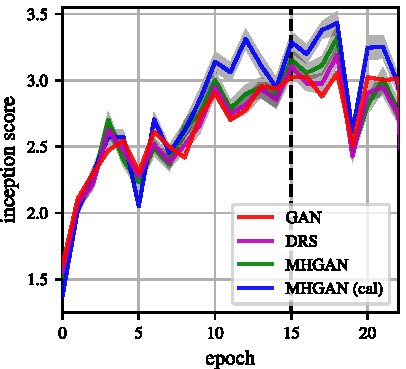
\includegraphics[width=2.2in]{figures/per_epoch_flat.pdf}
       \caption{performance by epoch}
       \label{fig:incep_by_epoch}
    \end{subfigure}
    \begin{subfigure}[b]{0.32\textwidth}
       \centering
       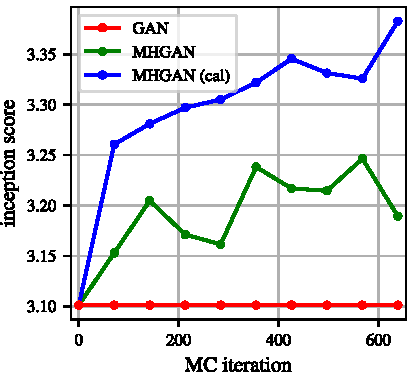
\includegraphics[width=2.2in]{figures/plot_per_mh_flat.pdf}
       \caption{performance by MCMC iteration}
       \label{fig:incep_by_iter}
    \end{subfigure}
    \begin{subfigure}[b]{0.32\textwidth}
       \centering
       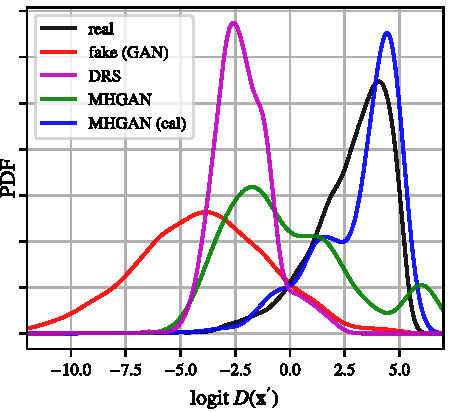
\includegraphics[width=2.2in]{figures/score_dist_bta_flat.pdf}
       \caption{epoch 13 scores}
       \label{fig:score_dist_overlap}
    \end{subfigure}
    \caption{{\small
    Results of the MH-GAN experiments on CIFAR-10 using the DCGAN\@.
     \textbf{(a)} On the left, we show the Inception score vs.~training epoch of the DCGAN with $k=640$ MH iterations.
    MH-GAN denotes using the raw discriminator scores and MH-GAN (cal) for the calibrated scores.
    The error bars on MH-GAN performance (in gray) are computed using a t-test on the variation per batch across 80 splits of the Inception score.
     \textbf{(b)} In the center we show the Inception score vs.~number of MCMC iterations $k$ for the GAN at epoch 15.
     \textbf{(c)} On the right, we show the scores at epoch 13 where there is some overlap between the scores of fake and real images.
    When there is overlap, the MH-GAN corrects the $\PG$ distribution to have scores looking similar to the real data.
    DRS fails to fully shift the distribution because 1)~it does not use calibration and 2)~its ``$\gamma$ shift'' setup violates the validity of rejection sampling.
    }}
    \label{fig:inception}
\end{figure*}
